\documentclass[10pt]{beamer}
 
\usepackage[T1]{fontenc}
\usepackage[utf8]{inputenc}
\usepackage{graphicx}
\usepackage{hyperref}
\usepackage{lmodern}
\usepackage{listings}
\usepackage{amssymb} 
\usepackage{xcolor}
\usetheme{Warsaw}
\usepackage{tikz}
\setbeamercovered{transparent}

\author{Latrille Thibault, Nicolas Lartillot, Laurent Duret}
\title{The red queen dynamic in the kingdom of recombination.}  
\institute{Laboratoire de Biométrie et Biologie Évolutive (LBBE), UMR CNRS 5558, Lyon}

\sloppy 

 
\begin{document}

\frame{\titlepage} 

\begin{frame}
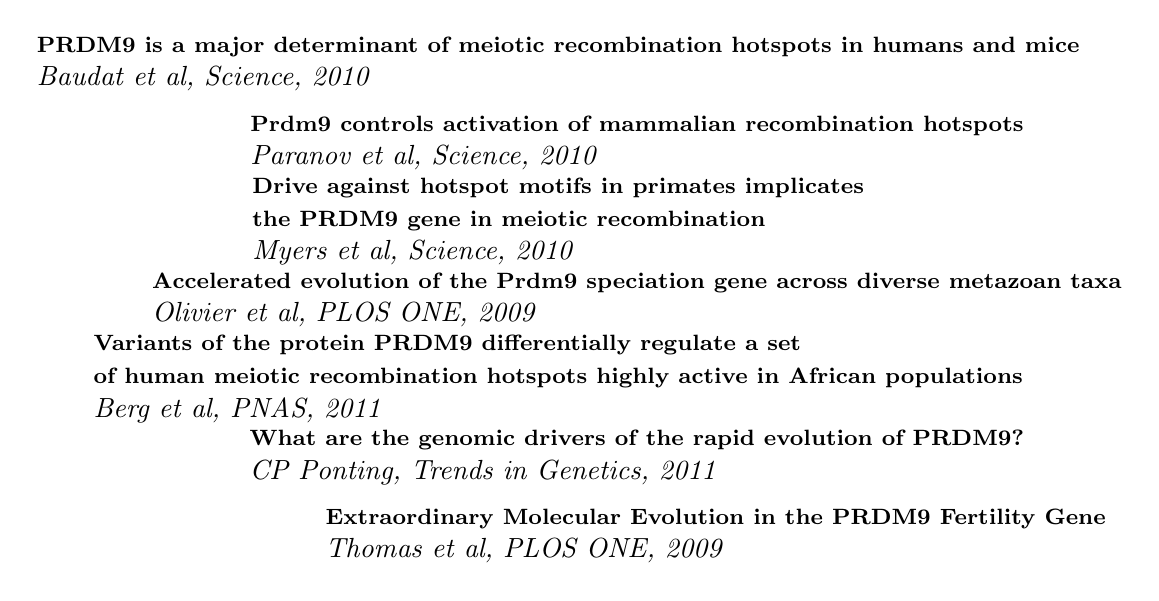
\begin{tikzpicture}
\node at (0,6) (A) [align=left] {\footnotesize \textbf{PRDM9 is a major determinant of meiotic recombination hotspots in humans and mice}\\\textit{Baudat et al, Science, 2010}};
\node at (1,5) (B) [align=left] {\footnotesize \textbf{Prdm9 controls activation of mammalian recombination hotspots}\\\textit{Paranov et al, Science, 2010}};
\node at (0,4) (C) [align=left] {\footnotesize \textbf{Drive against hotspot motifs in primates implicates} \\ \footnotesize \textbf{the PRDM9 gene in meiotic recombination}\\\textit{Myers et al, Science, 2010}};
\node at (1,3) (D) [align=left] {\footnotesize \textbf{Accelerated evolution of the Prdm9 speciation gene across diverse metazoan taxa}\\\textit{Olivier et al, PLOS ONE, 2009}};
\node at (0,2) (E) [align=left] {\footnotesize \textbf{Variants of the protein PRDM9 differentially regulate a set}\\\footnotesize \textbf{of human meiotic recombination hotspots highly active in African populations}\\\textit{Berg et al, PNAS, 2011}};
\node at (1,1) (F) [align=left] {\footnotesize \textbf{What are the genomic drivers of the rapid evolution of PRDM9?}\\\textit{CP Ponting, Trends in Genetics, 2011}};
\node at (2,0) (G) [align=left] {\footnotesize \textbf{Extraordinary Molecular Evolution in the PRDM9 Fertility Gene}\\\textit{Thomas et al, PLOS ONE, 2009}};
\end{tikzpicture}
\end{frame}

\begin{frame}
\frametitle{Overline of the presentation}
	\begin{center}
       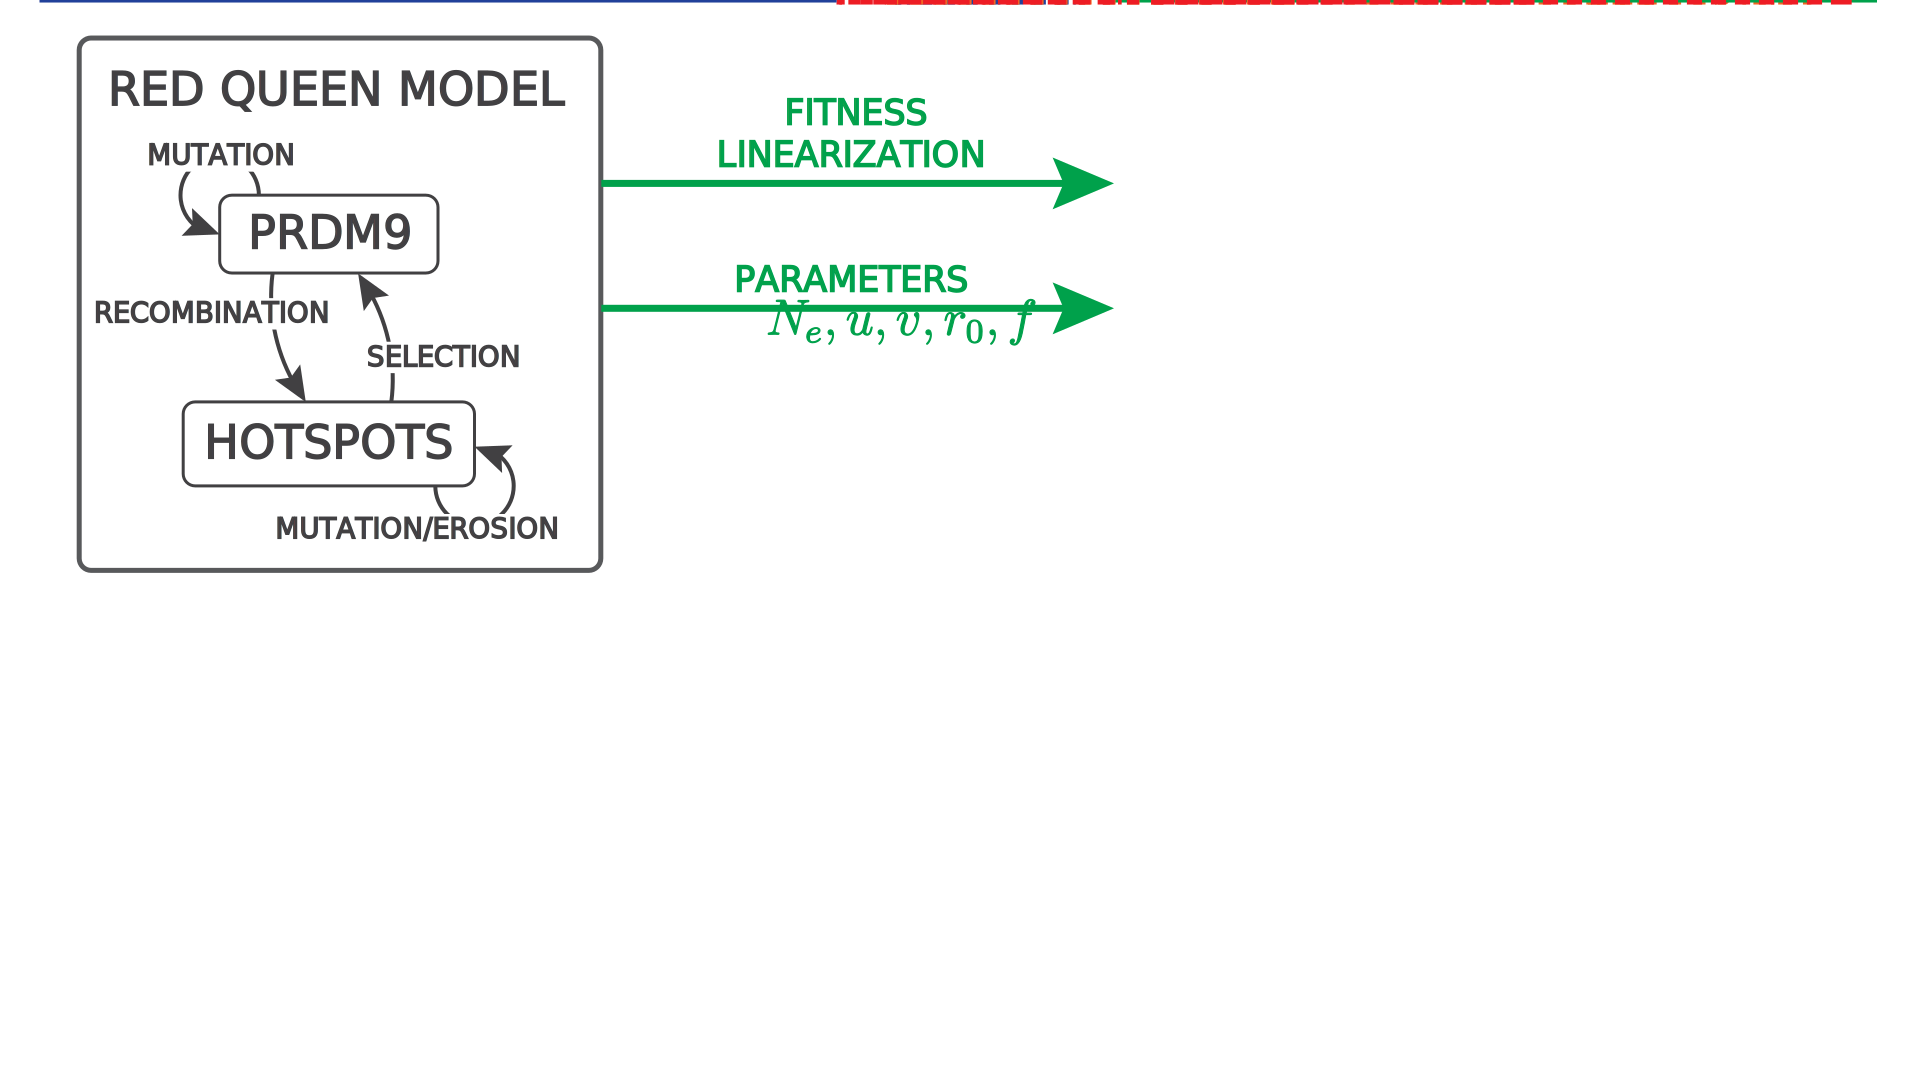
\includegraphics[width=8.5cm]{Images/overline.png}
	\end{center}
\end{frame}

\section{Red queen model}

\begin{frame}
	\begin{center}
	\huge
	Chapter 1. \\
       Red queen model
	\end{center}
\end{frame}

\begin{frame}
	\begin{center}
       \includegraphics[width=8.5cm]{Images/overline-1.png}
	\end{center}
\end{frame}

\begin{frame}
\frametitle{Recombination of the hotspots ruled by PRDM9}
	\begin{center}
       \includegraphics[width=9cm]{Images/RedQueen-1.png}
	\end{center}
\end{frame}

\begin{frame}
\frametitle{Erosion of the hotspots and selection of PRDM9}
	\begin{center}
       \includegraphics[width=9cm]{Images/RedQueen-2.png}
	\end{center}
\end{frame}

\begin{frame}
\frametitle{Mutation of PRDM9}
	\begin{center}
       \includegraphics[width=9cm]{Images/RedQueen-4.png}
	\end{center}
\end{frame}

\begin{frame}
\frametitle{Erosion, again and again...}
	\begin{center}
       \includegraphics[width=9cm]{Images/RedQueen-5.png}
	\end{center}
\end{frame}


\section{Population genetic model}

\begin{frame}
	\begin{center}
	\huge
	Chapter 2. \\
       Population genetic model
	\end{center}
\end{frame}

\begin{frame}
	\begin{center}
       \includegraphics[width=8.5cm]{Images/overline-2.png}
	\end{center}
\end{frame}

\begin{frame}
	\frametitle{Parameters}
	\begin{center}
       \includegraphics[width=9cm]{Images/red-queen-model.jpg}
	\end{center}
\end{frame}


\begin{frame}
	\frametitle{Parameters}
	\begin{center}
       \includegraphics[width=9cm]{Images/results.png}
	\end{center}
\end{frame}

\section{Results}

\begin{frame}
	\begin{center}
	\huge
	Chapter 3. \\
       Results
	\end{center}
\end{frame}


\begin{frame}
\frametitle{Results}
	\begin{center}
       \includegraphics[width=8.5cm]{Images/overline-3.png}
	\end{center}
\end{frame}

\begin{frame}
	\begin{center}
		\Large
    	Polymorphism of PRDM9
	\end{center}
	$ u $ is the mutation rate of PRDM9. \\
	$ N_e $ is the population size. \\ 
	\begin{enumerate}
		\item $u N_e \ll 1 \Rightarrow  $ single allele succession.
		\item $u N_e \gg 1 \Rightarrow  $ polymorphism.
		
		\item $\nearrow$ with regard to $u$ and $N_e$.
		
		\item $\rightsquigarrow$ with regard to the mutation and recombination rate at the hotspots.
		
		\item $\rightsquigarrow$ with regard to the fitness function.
	\end{enumerate}
\end{frame}

\begin{frame}
	\begin{center}
       \includegraphics[width=8.5cm]{Images/simpson-entropy-mutation-erosion.png}
	\end{center}
\end{frame}


\begin{frame}
	\begin{center}
       \includegraphics[width=8.5cm]{Images/simpson-entropy-population-erosion.png}
	\end{center}
\end{frame}

\begin{frame}
	\begin{center}
		\Large
    	Mean erosion of the hotspots
	\end{center}
	$ u $ is the mutation rate of PRDM9. \\
	$ N_e $ is the population size. \\ 
	$ v $ is mutation rate at the hotspots. \\
	$ r_0 $ is recombination rate of the hotspots. \\
	$ f $ is fitness function. \\
\end{frame}

\begin{frame}
	\begin{center}
       \includegraphics[width=8.5cm]{Images/mean-erosion-mutation-erosion.png}
	\end{center}
\end{frame}


\begin{frame}
	\begin{center}
       \includegraphics[width=8.5cm]{Images/mean-erosion-population-erosion.png}
	\end{center}
\end{frame}

\begin{frame}
	\begin{center}
		\Large
    	Cross-homozygosity of the hotspots
	\end{center}
	$ u $ is the mutation rate of PRDM9. \\
	$ N_e $ is the population size. \\ 
	$ v $ is mutation rate at the hotspots. \\
	$ r_0 $ is recombination rate of the hotspots. \\
	$ f $ is fitness function. \\
\end{frame}

\begin{frame}
	\begin{center}
       \includegraphics[width=8.5cm]{Images/cross-homozygosity-mutation-erosion.png}
	\end{center}
\end{frame}


\begin{frame}
	\begin{center}
       \includegraphics[width=8.5cm]{Images/cross-homozygosity-population-erosion.png}
	\end{center}
\end{frame}



\section{Single allele equations}

\begin{frame}
	\begin{center}
	\huge
	Chapter 4. \\
       Single allele equations
	\end{center}
\end{frame}


\begin{frame}
\frametitle{Single allele equations}
	\begin{center}
       \includegraphics[width=8.5cm]{Images/overline-4.png}
	\end{center}
\end{frame}

\begin{frame}
\frametitle{Single allele equations}
\begin{equation}
  \left\{
      \begin{aligned}
          \dfrac{\mathrm{d}x}{\mathrm{d}t} &= \dfrac{f'(\overline{L})}{2 f(\overline{L})} \left( l - \overline{L} \right) x \\
        \dfrac{\mathrm{d}l}{\mathrm{d}t} &= 
        - \rho x l \\
      \end{aligned}
    \right.
 \Rightarrow
  \left\{
      \begin{aligned}
          x(l) &=\dfrac{f'(\overline{L})}{2 \rho f(\overline{L})} (1-l + \overline{L} \mathrm{log}(l)) + x_{\mathrm{initial}} \\
        \dfrac{\mathrm{d}l}{\mathrm{d}t} &= 
         \dfrac{f'(\overline{L})}{2 f(\overline{L})} [ l-1- \overline{L} \mathrm{log}(l)]l  - \rho x_{\mathrm{initial}} l \\
      \end{aligned}
    \right.
\end{equation}
\end{frame}

\begin{frame}
\frametitle{Single allele equations}
	\begin{center}
       \includegraphics[width=11cm]{Images/SingleAllele.png}
	\end{center}
\end{frame}



\begin{frame}
\frametitle{Single allele equations}
	\begin{center}
       \includegraphics[width=8.5cm]{Images/overline-5.png}
	\end{center}
\end{frame}
\end{document}


